\chapter{Systembeschreibung}
\label{system}

Das nachfolgende Kapitel befasst sich mit der Beschreibung der Technologien und Vorgehensweisen, die zur Link Discovery im Rahmen dieser Arbeit angewendet wurden. Dazu zählen im Einzelnen die gewählte Datenbank MongoDB, das Datenmodell des Zielgraphen und die Beschreibung der implementierten Systemarchitektur zur Link Discovery.


\section{Systemarchitektur}

Nach erfolgter Technologieauswahl und Modellierung der Daten soll im nächsten Abschnitt die technische Umsetzung der Link Discovery beschrieben werden.

Da die Mongo Shell eine vollwertige JavaScript--Laufzeitumgebung enthält und skriptbar ist, wurden die meisten Operationen im Rahmen dieser Arbeit als Skripte für diese Shell implementiert. Einzig der Import der Tag-, Clicktracking- und Wortschatzdaten wurde mit Ruby--Skripten realisiert.

Die Schritte zur Link Discovery sind im Wesentlichen für jede zu integrierende Datenquelle gleich. Sie umfassen den Import, die Bereinigung, die Reduktion, die Transformation und die Integration der Daten \cite{hkp2012}.

\begin{figure}
\centering
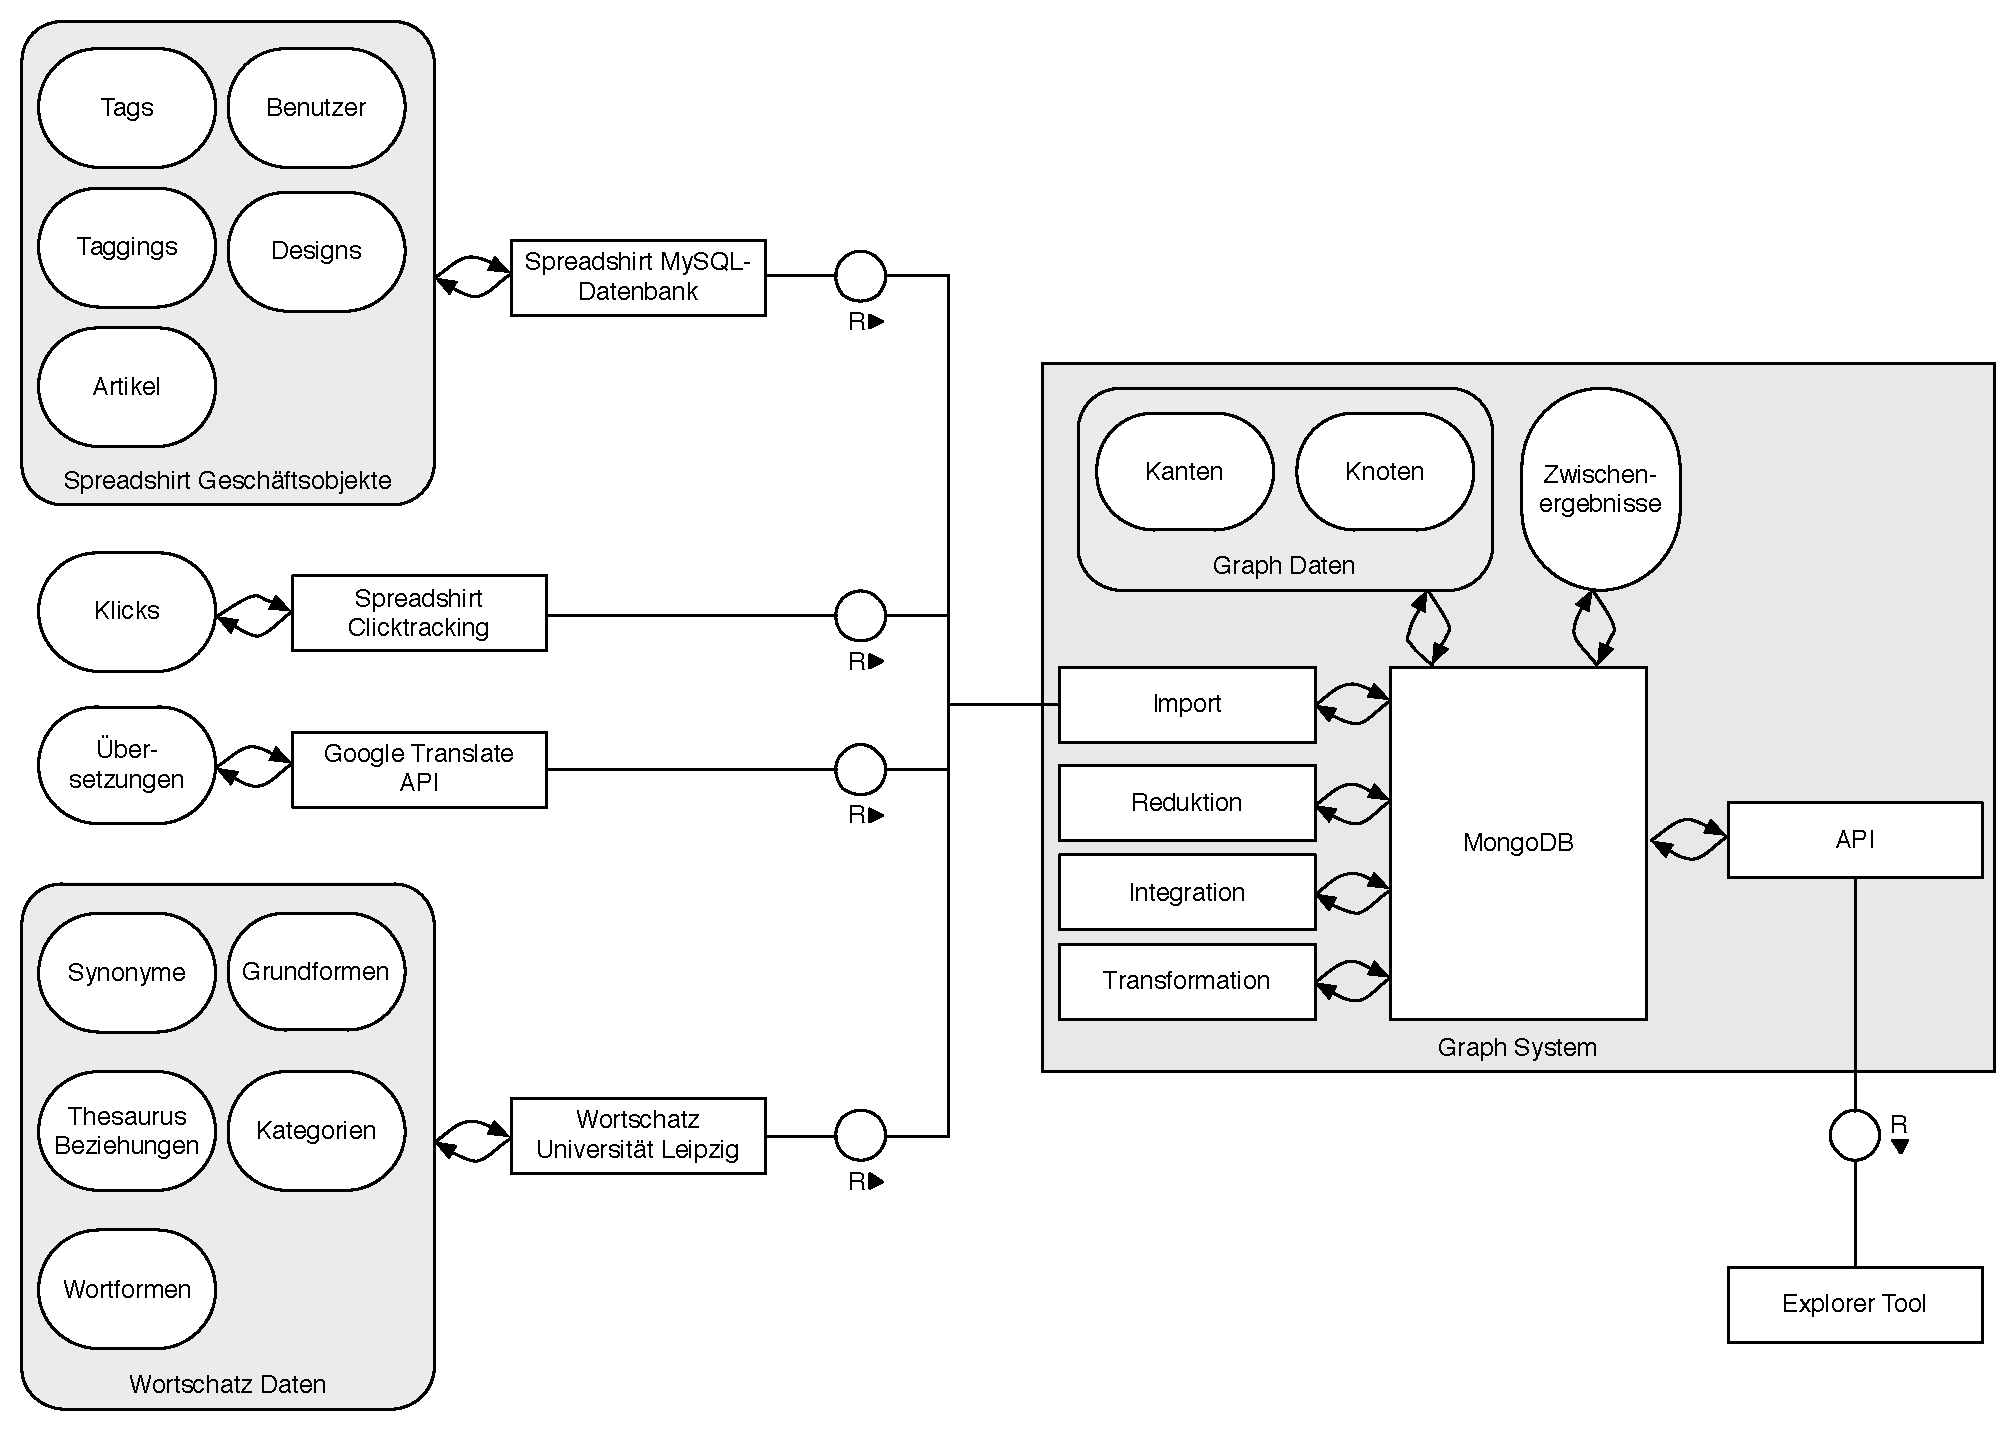
\includegraphics[width=1\textwidth]{architecture}
\caption{FMC--Blockdiagramm der gewählten Systemarchitektur}
\label{fig:architecture}
\end{figure}

\cref{fig:architecture} zeigt die komplette Architektur des implementierten Link Discovery Systems. Darin sind alle genutzten Datenquellen und die Daten, die sie bereit stellen, aufgeführt.

Für jede Datenquelle existiert ein Importskript, welches die Rohdaten importiert und in MongoDB speichert. Bei relationalen Datenquellen wie der MySQL--Datenbank von Spreadshirt für die Tag--Daten wird pro Tabelle eine Collection und pro Zeile ein Dokument angelegt. Können nicht alle Daten importiert werden, wie beispielsweise bei der Wortschatz--API (siehe \cref{wortschatz}, kann das Importskript auch aufgrund der bisher im Graph vorhandenen Daten eine Auswahl an Anfragen an die externe Datenquelle erzeugen.

Im nachfolgenden Bereinigungsschritt werden die Daten so gut wie möglich von eventuell vorhandenen Defekten befreit. Dazu zählen beispielsweise das Entfernen nicht nutzbarer Zeichen oder von unvollständigen Datensätzen.

Der Reduktionsschritt dient zur Verkleinerung der Datenmenge. Dazu gehören zum Beispiel Schritte zur Duplikatentfernung oder zur Auswahl relevanter Datensätze. In dieser Arbeit bestand die Haupteinschränkung der Datenmenge darin, nach Möglichkeit nur deutschsprachige Datensätze auszuwählen.

Der Schritt der Transformation überführt die Daten schließlich in eine Graphenform. Dies kann entweder über Kookkurrenz oder über eine andere, für die Art der importierten Daten geeignete, Methode erfolgen.

Das Integrationsskript für jede Datenquelle ist letztendlich für die Integration der Daten in den Zielgraphen verantwortlich. Dabei werden neue Knoten eingefügt, neue Informationen an vorhandene Knoten angefügt oder neue Kanten in den Graph integriert. In diesem Schritt passiert die Auflösung von eventuell vorhandenen temporären Bezeichnern in die entsprechenden im Graph vorhandenen eindeutigen Bezeichner.

Für die Abfrage der im Graph gespeicherten Informationen existiert außerdem eine API, welche Informationen zu Knoten und deren Nachbarn per HTTP als JSON--Dokumente zur Verfügung stellt. Diese API kann für die Einbindung der erzeugten Informationen in andere Applikationen genutzt werden. Über Anfrageparameter kann die Gewichtung der einzelnen Kantentypen beeinflusst werden.

Eine Beispielanwendung, die die API des Link--Discovery--Systems nutzt, ist der \emph{Tag Explorer}. Dabei handelt es sich um eine Browseranwendung, die die im Graph gespeicherten Beziehungen visualisiert und interaktiv erforschbar macht. Der Benutzer dieser Anwendung kann mit selbst gewählten Gewichtungen der Kanten den Graph durchsuchen. Außerdem werden, wenn vorhanden, über eine Anbindung der API von Spreadshirt zu der Zeichenkette des ausgewählten Knotens gefundene Designs angezeigt. In \cref{fig:tag_explorer} ist ein Screenshot dieses Werkzeugs zu sehen.

\begin{figure}
\centering
\includegraphics[width=\textwidth]{tag_explorer}
\caption{Tag Explorer}
\label{fig:tag_explorer}
\end{figure}

Nachdem das System zur Link Discovery in diesem Kapitel erläutert wurde, wird im nächsten Kapitel die praktische Durchführung und die Ergebnisse detailliert beschrieben.